\chapter{数学模型}
\label{cha:model}
根据地形数据作出该区域的等高线地形图如 所示
\begin{figure}[!ht]
\centering
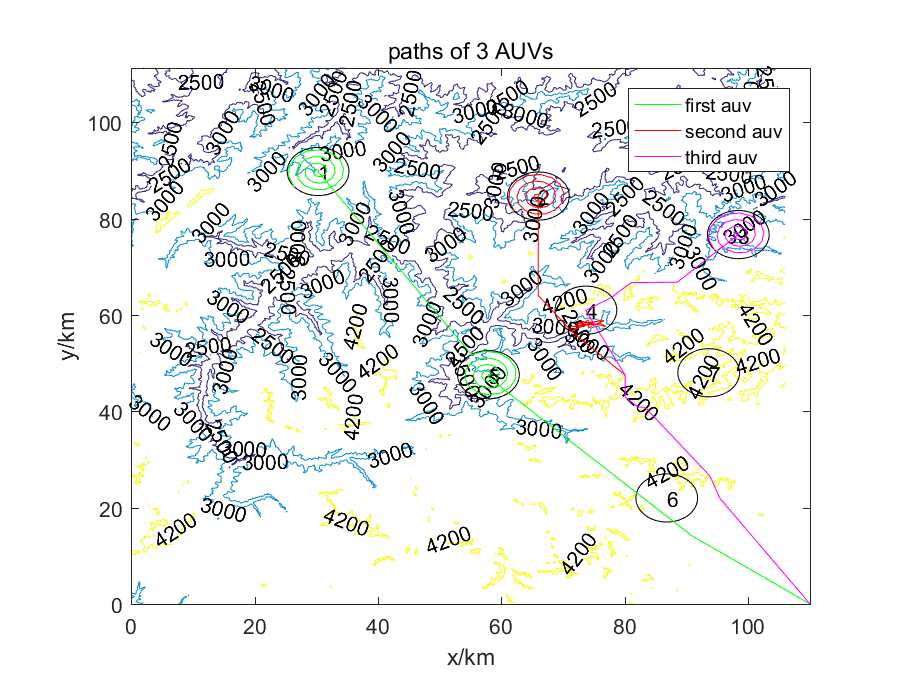
\includegraphics[width=18cm]{3path3.eps}
\caption{等高线地形图}\label{fig:3path}
\end{figure}

\section{模型假设}
\subsection{无人机路径规划算法选择}
对于单架无人机,希望其从指定起点到指点目标点的飞行时间最短。为此,我们将震区转化为二维网格,将高度超过4200米的地形区视为
障碍,在每一个网格的内部节点中,有8个相邻的节点,对于网格中的对角线的边,权值赋为$\sqrt{2}$,其余边为权值为1。
为此,我们给出如下的无人机路径规划方案:
\begin{enumerate}
\item 由震区地形数据建立图模型
\item 由图模型计算离散域的最短路径
\item 根据Visibility Graph 对离散域求出的最短路径进行优化并考虑到无人机飞行必须满足的约束条件对路径进行平滑
\end{enumerate}
\subsection{最大覆盖区域的优化算法选择}
最大覆盖区域的问题是NP难的问题,对于有高于4200米地形的重点区域,我们采用贪心算法对重点区域进行覆盖,该方法可在多项式时间内实现,
而且已有文献说明贪心法的平均覆盖率可达0.63\cite{Feige1998A}。贪心算法每次选取最低点并记录下已经巡逻到的区域,然后在未巡逻到3000米以下的区域
继续找最低点,直到巡逻区域在重点区域的比重达到设定的阀值。

在上述贪心方法找到若干个离散点后,若无人机遍历离散点,即可达到巡逻区域比例不低于上述阀值的效果。
为此,采用中国旅行商问题的思路规划出最短路径,求解中国旅行商问题采用整数规划的方法,并用增加不等式约束多次迭代
的方法消除子回路。由于离散点数目较少,完全图的规模较小,故该求解方法可行。
对于重点区域4使用上述方法求出20个圆的覆盖率达到$96\%$以上。并用整数规划的方法求出遍历这20个圆的圆心的
最短路径如图 \ref{fig:region4}所示
\begin{figure}[!ht]
\centering
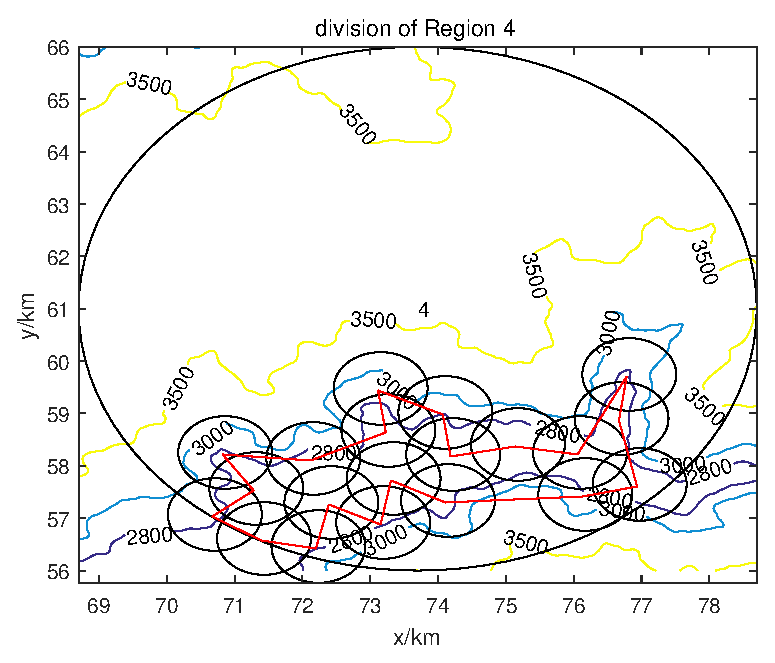
\includegraphics[width=10cm]{region4.eps}
\caption{重点区域4三千米以下位置的遍历路径}\label{fig:region4}
\end{figure}

对于全部低于4200米地形的重点区域,可以实现全覆盖。为此我们先让无人机飞到目标区域的圆心,
并采用阿基米德螺旋线的方式进行巡查。由于阿基米德螺旋线具有从起点出发的射线与螺旋线交点等距的性质,相比其它飞行轨迹
实现全覆盖用时较短。
以螺旋线起点为极坐标原点,则旋线方程为:
\begin{equation}
r=b\theta
\end{equation}
分隔距离为
\begin{equation}
d=2\pi b
\end{equation}
对于低于4200米地形区域(A,B,C,E)之一,记其最大高度为$h_g$,无人机飞行高度记为$h_a$, 则覆盖半径的最小值为
\begin{equation}
r_{\text{min}}=\tan(\phi_e/2)(h_a-h_g)
\end{equation}
取 $d=2r_{\text{min}}$ 可保证无人机按螺旋线飞行可实现自圆心向外区域的全部覆盖。无人机飞行所需的最小角度为
\begin{equation}\label{eq:thetaMin}
\theta_{\text{min}}=\frac{r_i-r_{\text{min}}}{b}
\end{equation}

%为保证螺旋线转过第一个$360^{\circ}$时可以覆盖图(\ref{fig:SpiralCenter})所示的区域,要求
%\begin{figure}[!ht]\label{fig:SpiralCenter}
%\centering
%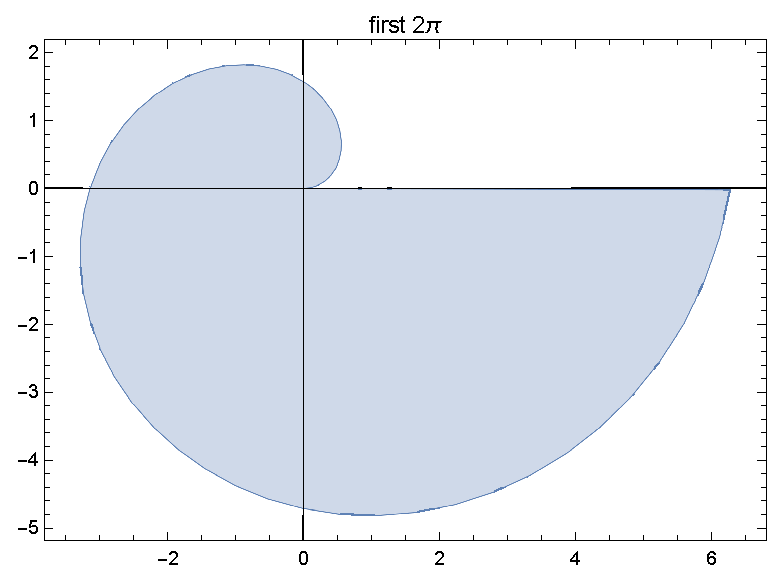
\includegraphics[width=6cm]{spiralCenter.eps}
%\caption{$r\leq b,\theta\leq 2\pi$}
%\end{figure}
为保证无人机转弯半径的要求,即螺旋线上任一点的曲率半径$\rho$大于$r_t$,即
\begin{equation}
\frac{b(\theta^2+1)^{\frac{3}{2}}}{\theta^2+2}\geq r_t
\end{equation}
对于螺旋线,我们取$\theta$从$\pi$开始,上式约束即为:
\begin{equation}
\frac{b(\pi^2+1)^{\frac{3}{2}}}{\pi^2+2}\geq r_t
\end{equation}
而对于$[0,\pi]$之间的飞行曲线,由于距离较短,无人机可调整方向进入螺旋线轨道。用时按$\frac{b\pi}{v_a}$近似。
根据螺旋线的弧长公式
\begin{equation}
s(\theta)=\frac{1}{2}b(\theta\sqrt{1+\theta^2}+\sinh^{-1}\theta)
\end{equation}
代入\eqref{eq:thetaMin}中的最小角度即可求出最小飞行距离$s_{\text{min}}$,除以无人机的速度$v_a$即可得飞行时间。
%关于极轴方向选取的任意性。
\section{实际计算中的近似}
%计算覆盖区域时做的近似:
\begin{itemize}
\item 无人机飞行折线的近似
\item 路径规划问题转化为图模型时只考虑无人机沿坐标轴与对角线方向的飞行
\item 只按最大俯角计算覆盖区域时忽略了能见范围内可能存在的地形遮挡
\end{itemize}
\subsection{平滑算法}
对于无人机飞行折线的近似,在所有折线的拐角处,我们按拐角的大小分如下两种情况对飞行曲线进行平滑以满足最小飞行半径的要求:
$\theta<80^{\circ}$,这时飞机曲线转弯用时比折线用时更长,多出的时间为
\begin{equation}
\Delta t=r_t(\pi+\theta-\tan\theta)
\end{equation}
示意图如下:
\begin{figure}[!ht]\label{fig:smaller}
\centering
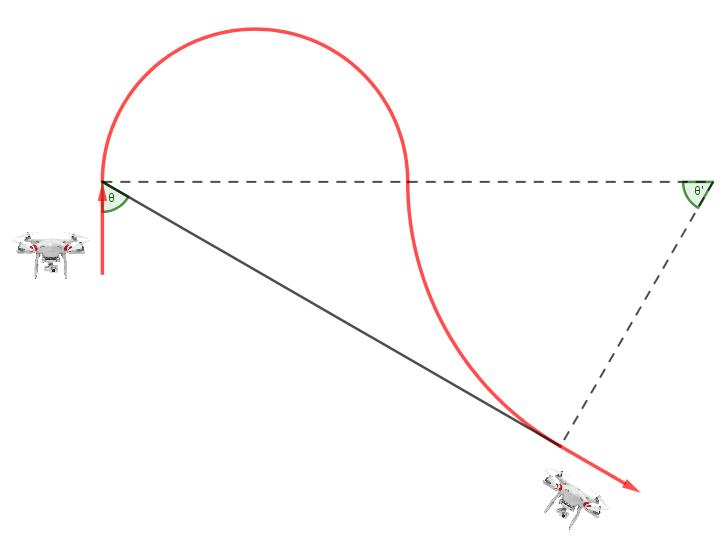
\includegraphics[width=6cm]{smaller.jpg}
\caption{$\theta<80^{\circ}$}
\end{figure}

$\theta>80^{\circ}$,用外接圆弧对折线进行平滑,这时飞机曲线转弯用时比折线用时更短$\Delta t<0$,
\begin{equation}
\Delta t=r_t(\frac{2}{\tan (\theta/2)}-\pi+\theta)
\end{equation}
示意图如下:
\begin{figure}[!ht]\label{fig:larger}
\centering
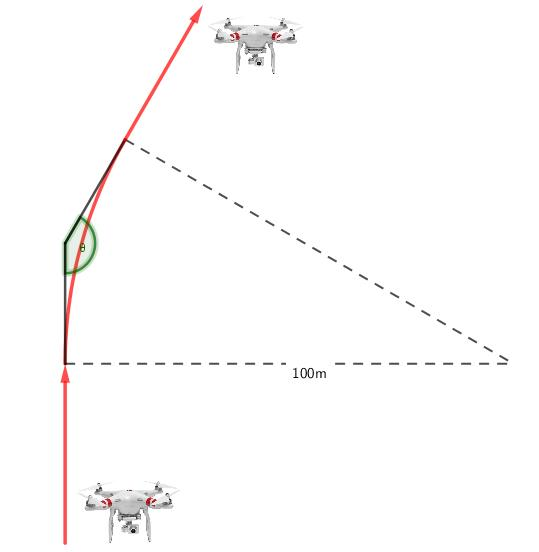
\includegraphics[width=6cm]{larger.jpg}
\caption{$\theta>80^{\circ}$}
\end{figure}

\subsection{Theta Star 算法}
我们在路径规划中,使用dijkstra 算法求图中两点的最短路径。理论上原问题中任意可直达的两点均需转化为一条边,且需要全局考虑。
但这样做计算开销过大,因此我们采用只考虑正方形边和对角线的方式,这样求出的图中的最短路径并非是原问题的最短路径,因为这时的路径的
方向角只能取 $0,45^{\circ},90^{\circ},135^{\circ}$ 这几个有限的值。我们针对求出的路径进行后处理,通过对路径的折线拐点根据是否可直达
重建一个小规模的图再次使用dijkstra 算法求最短路径,从而大幅减少了最终折线拐点的数量。

关于判断地图中两点是否可直达的算法,我们借用计算机图形学在栅格点画直线的方法\cite{Bresenham1965Algorithm},可避免浮点数运算,时间复杂度是$O(n)$。

针对图中的最短路径并非是原问题的最短路径这一问题,文献\cite{Nash2014Theta} 给出了一种在规划最短路径时不局限于图的边的方法,以取代A star等方法需要
后处理的随意性,在我们的模型中,我们也考虑使用 Theta Star 算法,由于整个算法用matlab 纯脚本实现,难以使用优先队列等数据结构对算法进行优化,
因此对于规模较大的问题运算过慢,这里只作为一种替代方法提出。

\subsection{地形遮挡}
给定无人机的空间位置求解其覆盖区域时,我们采用的是比较无人机附近的点的圆锥投影侧面上的点是否在地形之上的方法。这样做避免了空间上判断
视距的问题,使单次判别的复杂度由$O(n)$降到$O(1)$,但有可能忽略了中间的地形遮挡而存在误判,考虑到地形起伏的连续性及问题的实际参数,误判相对较小,因此我们采用
锥面投影的方法作为求覆盖区域的主要方法。

根据上面的说明,我们计算出重点区域4,6内没有3000米以下的地方,因此无人机无需飞往。
对于其他5个重点区域,至少需要3架无人机可使全部重点区域的3000米以下的地方覆盖率达到$100\%$,
其飞行路线如图 \ref{fig:3path} 所示,其中第一架无人机负责巡逻区域5和区域1,
用时3.82小时;第二架无人机负责巡逻区域4和区域2,用时3.14小时;第三架
无人机负责巡逻区域3,用时2.66小时。

\section{区域全部覆盖时的补充}
\subsection{稀疏采样}
求解全部覆盖区域时由于格点过密,难以全局直接用图论的方法求解。我们首先根据无人机的覆盖区域对整个区域进行重采样,得到原格点数$\frac{1}{25}$的样本点,
若多架无人机全部遍历这些点,则可实现对整个区域的覆盖。

针对全部求出的点,可以采用 VRP (Vehicle Routing Problem) 的方法对给定的无人机数量进行路径规划。由于时间和能力所限,
我们在这方面仅仅做了一些文献调研并提出一些初步的设想:

对于大规模的VRP问题,难以精确求解,需要采用近似算法,如遗传算法或模拟退火\cite{Kirkpatrick1983Optimization}的方法,
其中模拟退火的方法从一组可行解出发,通过随机选取这组可行解的邻居解,通过比较两组解对应的代价函数的大小按一定概率
决定是否进行状态转移,由于本问可行解不易构造,由于地形的限制,邻居解难以刻画,故我们暂时没有想到如何求解该问题。

